\documentclass[18pt,caption=numbered]{beamer}
\usetheme[color=screen]{UniBern}

\usepackage{lmodern}
\usepackage[english]{babel}
\usepackage{microtype}
\usepackage{textcomp}
\usepackage[backend=biber,natbib=true, sorting=none, url=false]{biblatex}
\addbibresource{~/Documents/library.bib}
\usepackage{graphicx}
\usepackage{tikz}
\usepackage[detect-all=true]{siunitx}
\usepackage{csquotes}
\usepackage{animate}
\usepackage{booktabs}
\usepackage[absolute,overlay]{textpos} %for the \source{} command
\usepackage{gitinfo2}
\usepackage{hyperref}

\hypersetup{pdfstartview={Fit}}
\setbeamertemplate{caption}{\insertcaption}
\setbeamertemplate{caption}[numbered]

\newcommand{\imsize}{\linewidth}
\newlength\imagewidth % needed for scalebars
\newlength\imagescale % ditto

\subtitle{Bruker microCT SkyScan 1172 \& 1272}
\author{David Haberthür}
\institute{Institute of Anatomy\\Universität Bern}
\date{19. August 2016\\Meeting mit Klaus Weber (Anapath)}

\begin{document}
\title{Was können unsere \si{\micro}CT-Maschinen?} % http://tex.stackexchange.com/a/144445/828

\begin{frame}
	\maketitle
\end{frame}

\begin{frame}
	\frametitle{Tumor load in lungs}
	\begin{itemize}
		\item Collaboration with DKF
		\item KP-TNIK influences tumor load
		\item Critical point dried lungs		
	\end{itemize}
\end{frame}

\end{document}

\begin{frame}
	\frametitle{Tumor load in lungs}
	\animategraphics[palindrome,width=325]{12}{../../Documents/Collaborations/DKF_Lung/movieframes/out-}{001}{255}
\end{frame}

\end{document}
\begin{frame}
	\renewcommand{\imsize}{0.33\linewidth}	
	\frametitle{Tumor load in lungs | Top: KO, bottom: WT}	
	\centering
	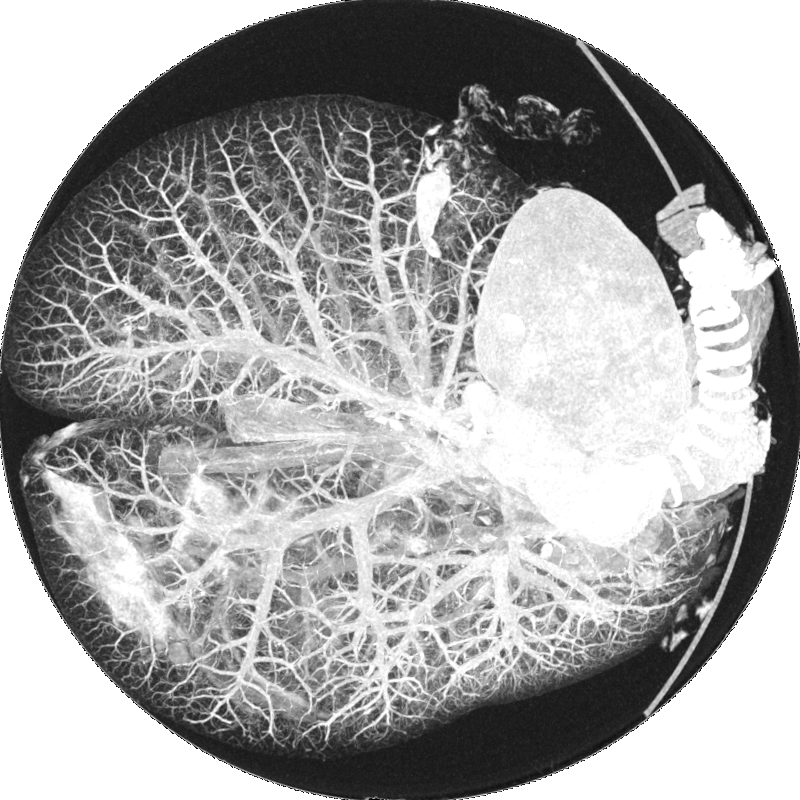
\includegraphics[width=\imsize]{../../Documents/Collaborations/DKF_Lung/Overview/MAX_--11.png}%
	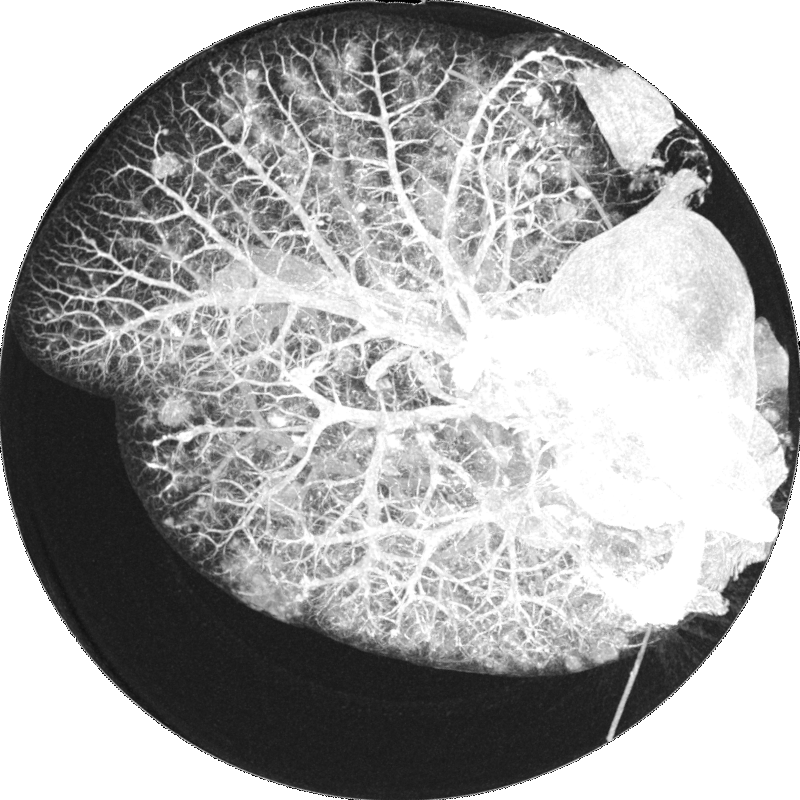
\includegraphics[width=\imsize]{../../Documents/Collaborations/DKF_Lung/Overview/MAX_--12.png}%
	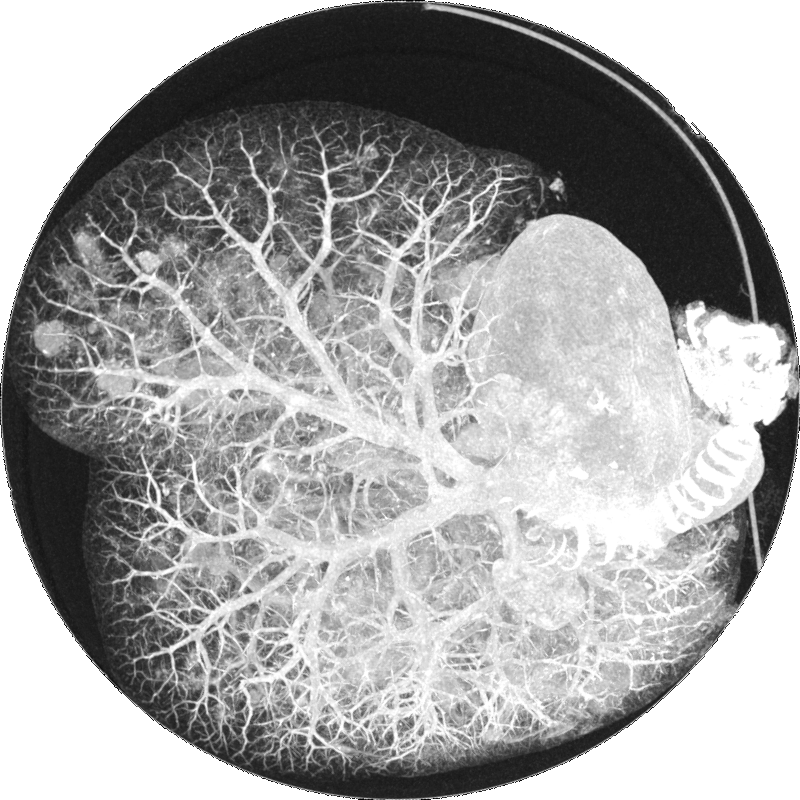
\includegraphics[width=\imsize]{../../Documents/Collaborations/DKF_Lung/Overview/MAX_--13.png}\\%
	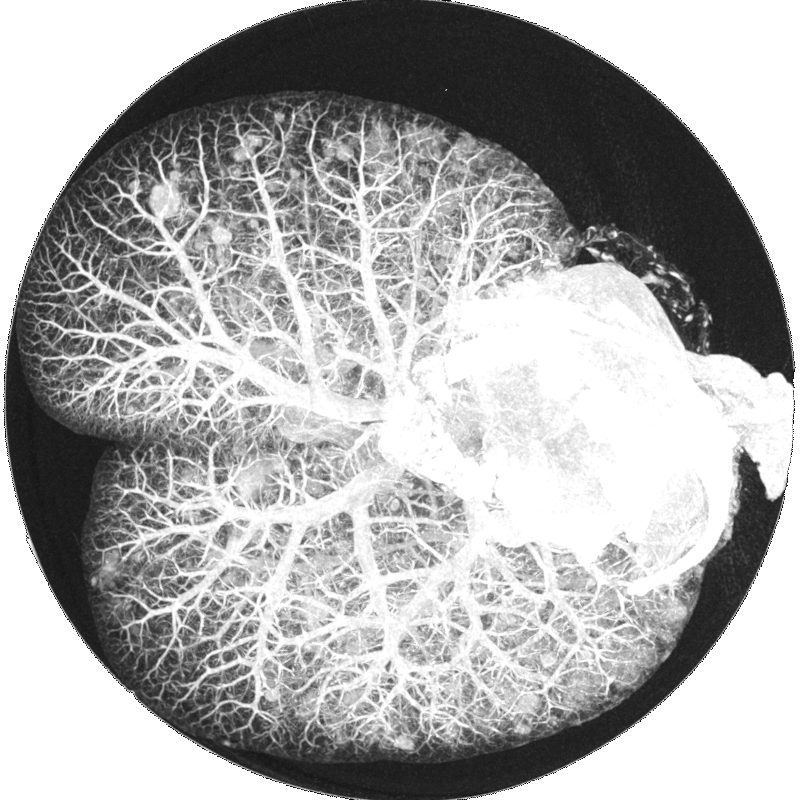
\includegraphics[width=\imsize]{../../Documents/Collaborations/DKF_Lung/Overview/MAX_wt11.png}%
	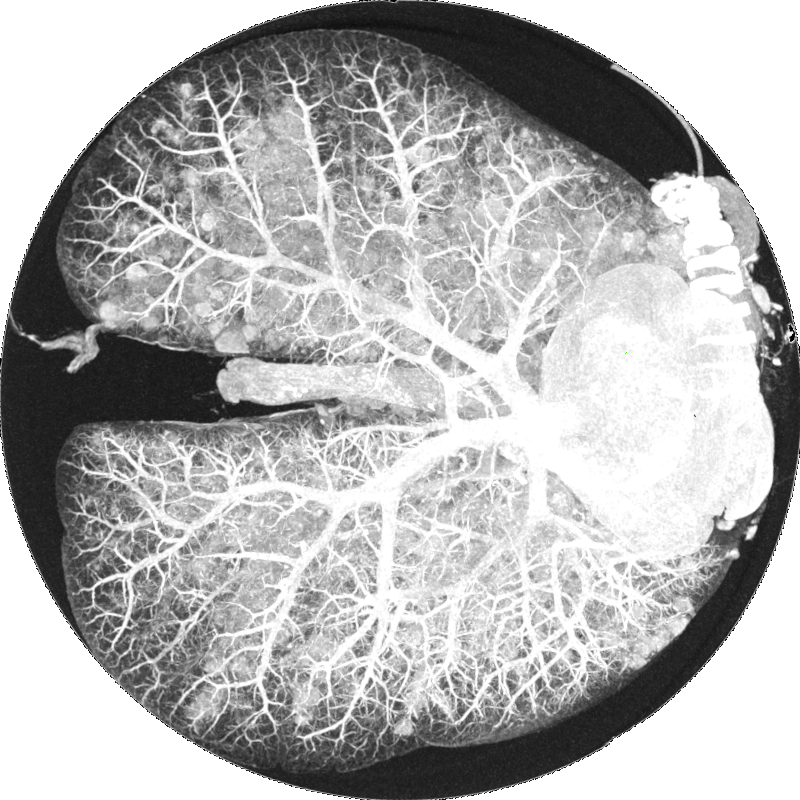
\includegraphics[width=\imsize]{../../Documents/Collaborations/DKF_Lung/Overview/MAX_wt12.png}%
	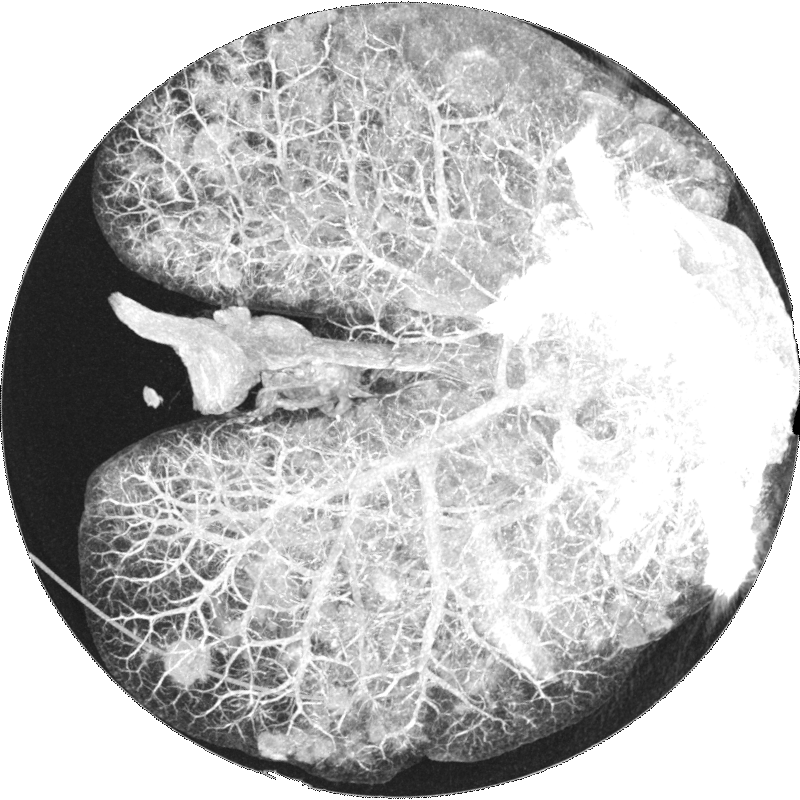
\includegraphics[width=\imsize]{../../Documents/Collaborations/DKF_Lung/Overview/MAX_wt13.png}%
\end{frame}

\begin{frame}
	\frametitle{Tumor metastasis\\Overview scan (\SI{20}{\micro\meter} voxel size)}
	\centering
	\animategraphics[palindrome,width=275]{12}{img/tumor/mouse_tumor_rec0}{001}{263}
\end{frame}

\begin{frame}
	\renewcommand{\imsize}{\linewidth}	
	\frametitle{Tumor metastasis\\Reconstruction (\SI{3}{\micro\meter} voxel size)}	
	\centering	
	\pgfmathsetlength{\imagewidth}{\imsize}%
	\pgfmathsetlength{\imagescale}{\imagewidth/4904}%
	\def\x{3031}% scalebar-x starting at golden ratio of image width of 4904px = 3031
	\def\y{2140}% scalebar-y at 90% of image height of 2378px = 2140
	\begin{tikzpicture}[x=\imagescale,y=-\imagescale]
		\node[anchor=north west, inner sep=0pt, outer sep=0pt] at (0,0) {\includegraphics[width=\imagewidth]{img/{{KP-TNIPWT13_rec00004162}}}};
		% 4904px = 14.712mm > 100px = 300um > 167px = 500um, 33px = 100um
		\draw[|-|,white,thick] (\x,\y) -- (\x+167+167,\y) node [midway,above] {\SI{1}{\milli\meter}};
	\end{tikzpicture}%
\end{frame}

\end{document}